\documentclass[12pt, twoside]{article}
\usepackage[letterpaper, margin=1in, headsep=0.5in]{geometry}
\usepackage[english]{babel}
\usepackage[utf8]{inputenc}
\usepackage{amsmath}
\usepackage{amsfonts}
\usepackage{amssymb}
\usepackage{tikz}
\usetikzlibrary{quotes, angles}
\usepackage{graphicx}
\usepackage{multicol}

%\usepackage{pgfplots}
%\pgfplotsset{width=10cm,compat=1.9}
%\usepgfplotslibrary{statistics}
%\usepackage{pgfplotstable}
%\usepackage{tkz-fct}
%\usepackage{venndiagram}

\usepackage{fancyhdr}
\pagestyle{fancy}
\fancyhf{}
\renewcommand{\headrulewidth}{0pt} % disable the underline of the header

\fancyhead[RE]{\thepage}
\fancyhead[RO]{\thepage \\ Name: \hspace{3cm}}
\fancyhead[L]{BECA / Dr. Huson / Geometry 10th Grade\\* Unit 1: Introduction to Geometry\\27 September 2019}

\begin{document}
\subsubsection*{2.9 Homework: Calculations in geometry}
  \vspace{0.25cm}
  \begin{enumerate}

  \item Given $\overline{ABC}$, $BC=36.9$, and $AC=87.3$.\\ [0.5cm]
  Find ${AB}$.\\[1.5cm]
      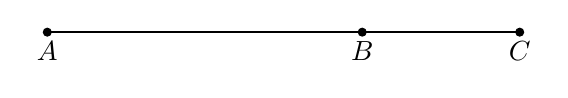
\begin{tikzpicture}
        \draw [-, thick] (1,0)--(7,0);
        \draw [fill] (1,0) circle [radius=0.05] node[below]{$A$};
        \draw [fill] (5,0) circle [radius=0.05] node[below]{$B$};
        \draw [fill] (7,0) circle [radius=0.05] node[below]{$C$};
      \end{tikzpicture} \vspace{1cm}

  \item Given $\overline{DEF}$, $DF=75$ and $\overline{DE}$ is half the length of $\overline{EF}$. \\ [0.25cm]
  Find ${DE}$.\\[.5in]
      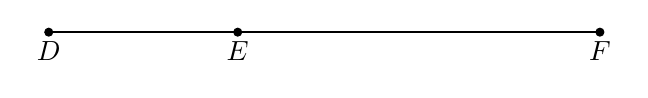
\begin{tikzpicture}
        \draw [-, thick] (1,0)--(8,0);
        \draw [fill] (1,0) circle [radius=0.05] node[below]{$D$};
        \draw [fill] (3.4,0) circle [radius=0.05] node[below]{$E$};
        \draw [fill] (8,0) circle [radius=0.05] node[below]{$F$};
      \end{tikzpicture} \vspace{2.5cm}

    \item Given $\overleftrightarrow{PQ}$ as shown on the number line. Divide segment $\overline{PQ}$ into five congruent segments by marking and labeling the points $R$, $S$, $T$, and $U$ on the numberline.\\[20pt] % Midpoint
    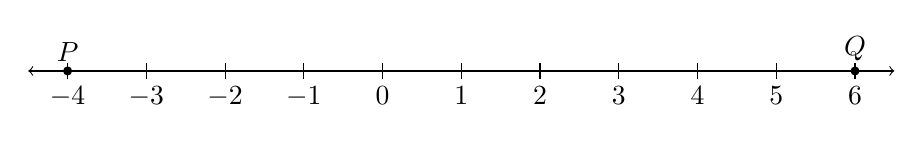
\begin{tikzpicture}
      \draw [<->] (-4.5,0)--(6.5,0);
      \foreach \x in {-4,...,6} %2 leading for diff!=1
        \draw[shift={(\x,0)},color=black] (0pt,-3pt) -- (0pt,3pt) node[below=5pt]  {$\x$};
        \draw [fill] (-4,0) circle [radius=0.05] node[above] {$P$};
        \draw [fill] (6,0) circle [radius=0.05] node[above] {$Q$};
    \end{tikzpicture}

    \item Given $\overleftrightarrow{RS}$ as shown on the number line, with $R=-2.8$ and $S=4.4$. \\[5pt]
    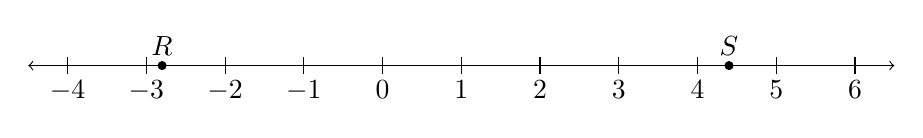
\begin{tikzpicture}
      \draw [<->] (-4.5,0)--(6.5,0);
      \foreach \x in {-4,...,6} %2 leading for diff!=1
        \draw[shift={(\x,0)},color=black] (0pt,-3pt) -- (0pt,3pt) node[below=5pt]  {$\x$};
        \draw [fill] (-2.8,0) circle [radius=0.05] node[above] {$R$};
        \draw [fill] (4.4,0) circle [radius=0.05] node[above] {$S$};
    \end{tikzpicture} \\ 
    The points $T$ and $U$ trisect $\overline{RS}$. Find their values, and mark and label them on the numberline. \vspace{4cm}

\newpage
    \item The rectangle $ABCD$, shown below, has a perimeter of 42, and $AB=13$. Find the area of the rectangle.
    \begin{flushleft}
    \begin{tikzpicture}[scale=0.8]
      \draw [-, thick] (0,0)--(7,0)--(7,4)--(0,4)--cycle;
      \draw [fill] (0,0) circle [radius=0.05] node[left]{$A$};
      \draw [fill] (7,0) circle [radius=0.05] node[right]{$B$};
      \draw [fill] (7,4) circle [radius=0.05] node[right]{$C$};
      \draw [fill] (0,4) circle [radius=0.05] node[left]{$D$};
      %\node at (-0.5, 2){5};
      \node at (3.5, -0.5){13};
    \end{tikzpicture}
    \end{flushleft}

    \item Given the rectangle $HOLA$ shown below, with length $HO=12.6$. The width $AH$ is one-half of the length $HO$. Find the perimeter of the rectangle.
    \begin{flushleft}
    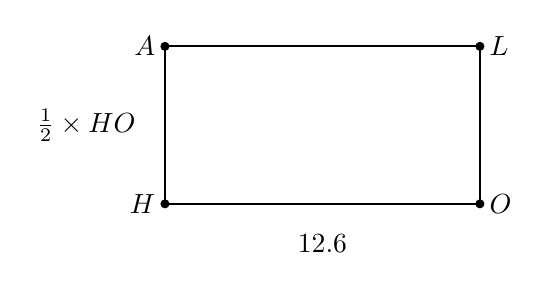
\begin{tikzpicture}
      \draw [-, thick] (0,0)--(4,0)--(4,2)--(0,2)--cycle;
      \draw [fill] (0,0) circle [radius=0.05] node[left]{$H$};
      \draw [fill] (4,0) circle [radius=0.05] node[right]{$O$};
      \draw [fill] (4,2) circle [radius=0.05] node[right]{$L$};
      \draw [fill] (0,2) circle [radius=0.05] node[left]{$A$};
      \node at (-1, 1){$\frac{1}{2} \times HO$};
      \node at (2, -0.5){12.6};
    \end{tikzpicture}
    \end{flushleft}
    \vspace{3cm}

    \item In the following two problems, solve for the value of $x$.
  \begin{multicols}{2}
    \begin{enumerate}
      \item   $\frac{2}{7}(16x+5)=10 \frac{4}{7}$ \vspace{6cm}
      \item   $x^2-8x-9=0$ \vspace{6cm}
    \end{enumerate}
  \end{multicols}
    \vspace{3cm}


  \end{enumerate}
\end{document}
